\documentclass{article}
\usepackage{amsmath}
\usepackage{amssymb}
\usepackage{algpseudocode}
\usepackage{algorithm}
\usepackage{graphicx}
\usepackage{caption}
\usepackage{subcaption}
\usepackage{float}


\begin{document}
\title{Homework 1 - CMSC-25400}
\author{Patrick Collins}
\date{\today}
\maketitle

\section{Proofs}
\begin{enumerate}
\item Derive an algorithm that can learn any monotone conjunction over
  ${0, 1}^n$ with a mistake bound of $n$. \\

\begin{algorithm}
\caption{Addition for Monotone Conjunctions}
\begin{algorithmic}[1]
\State $f \gets \bigwedge\limits_{n=1}^n x_n$
\State $i \gets 1$
\While{True}
\State predict $\hat{y}^t = f(x^t)$
\If{$(\hat{y}^t == 1)$ and $(y^t == 0)$}
\State remove $\{x | x \in x^t$ if $x == 1$\} from $f$.
\EndIf
\State $t \gets t + 1$
\EndWhile
\end{algorithmic}
\end{algorithm}

Proof of mistake bound:

Note that: (a) this algorithm will only ever produce false
negatives, and (b) it removes at least one term from the
concept for every false negative. Therefore, because there are only
$n$ terms total, it can make a maximum of $n$ mistakes. 

\item Prove that, for any concept class $C$ and online algorithm $A$
  with finite mistake bound $M$, there is a conservative algorithm
  $A'$ with mistake bound $M$ on $C$. 

Suppose that there exists some algorithm $A$ that can select a true
hypothesis from concept class $C$ with a mistake bound of
$M$. Consider an arbirary set of training inputs, $x^1,
x^2,\dots,x^n$, and let $x^i$ be the training input where $A$ develops a true
hypothesis. Consider $x^j$, the last input for which $A$ makes a
mistake. It must be the case that $j \leq i$, since, if $A$ already had a
true concept, it would no longer make mistakes. 

Suppose $j < i$. Then there exists some series of inputs $x^{j+1},
x^{j+2},\dots,x^{i-1}$ such that $A$ provides the correct answer for
each. By assumption, it is also true that $A$ provides the correct
answer for $x^i,\dots$ But if $A$ provides the correct answer for all
inputs after $x^j$, then it must be the case that $A$ has a true
concept at $x^j$, therefore $i = j$. 

Therefore, there exists an $A'$ such that $A'$ has a mistake bound $M$
on $C$ and $A'$ is conservative.

\item 

\item Results from applying KMeans:

\begin{figure}[H]
  
\includegraphics{../output/small.png}
\end{figure}
\begin{figure}[H]
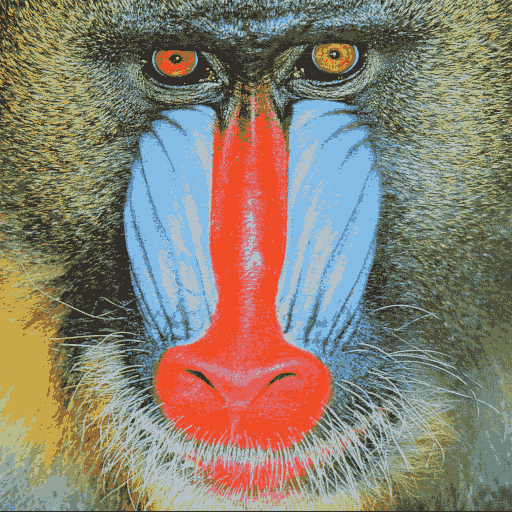
\includegraphics{../output/large.png}
\end{figure}

\pagebreak
The contrast in the resulting, compressed image is sharper, reflecting
the fact that the number of colors in the pictures has been halved. It
also appears to be somewhat more washed-out than the original.

This compression reduces the total number of colors to 16, meaning
that each pixel can be represented with three 4-bit numbers rather
than 8-bit ones, resulting in a compression ratio of approximately
50\% for large images, because the storage requirement for each pixel
has been halved. 




\end{enumerate}
\end{document}
